\chapter{Descriptive Statistics and Visualization}\label{Chapter:DescriptiveVisualization}

\newthought{This chapter} presents two closely related sets of operations:
descriptive statistics and visualization.
The former aims at extracting valuable information, both numerical and graphical, with the least possible hypotheses about the data.
The latter gathers techniques for presenting the data as images which reveal interesting features about the scene under analysis.

\section{Descriptive Statistics}

Bearing in mind the strong connection SAR data have with their statistical properties, it is highly recommended to start handling such data as a sample. This section presents the main tools every SAR data analyst should be comfortable to use and exploit.

We will use two data sets: \texttt{dark.Rdata} and \texttt{bright.Rdata}, which were extracted from the image shown in Fig.~\ref{Im:Oberpfaffenhofen_RGB} (page~\pageref{Im:Oberpfaffenhofen_RGB}, the yellow and red areas, respectively).
Each data set is comprised of three bands: HH, HV and VV.

The first operation should always consist in checking the size and type of data:
\begin{lstlisting}
> dim(dark)
[1]  63 247   3
> typeof(dark)
[1] "double"
\end{lstlisting}
With this we know the data is arranged in three bands of \num{63} lines and \num{247} columns each, and that these are double precision floating records.

It is convenient to organize the data as a \texttt{data.frame}
\begin{lstlisting}
dark_data.frame <- data.frame(HH=as.vector(dark[,,1]),
 HV=as.vector(dark[,,2]), 
 VV=as.vector(dark[,,3]))
\end{lstlisting}

And now we can apply the \texttt{summary} function:
\begin{lstlisting}
> summary(dark_data.frame)
             HH                  HV                  VV
 Min.   :     1   Min.   :    0.004   Min.   :     0.17  
 1st Qu.:  1821   1st Qu.:  134.675   1st Qu.:   950.78  
 Median :  4414   Median :  326.652   Median :  2364.09  
 Mean   :  7552   Mean   :  509.596   Mean   :  3882.10  
 3rd Qu.:  9060   3rd Qu.:  662.560   3rd Qu.:  4957.64  
 Max.   :526287   Max.   :15723.672   Max.   :134204.69  
\end{lstlisting}

We immediately notice the different ranges: the observations in the HV band are one order of magnitude smaller than those in the other bands.

The histograms of these bands were shown in Fig.~\ref{Fig:FittedDarkRegion}.
Another useful representation of the marginal distribution of the data is the boxplot.

A boxplot is a graphical representation of the marginal properties of the data.
It depicts the median, the lower and upper quartiles, and possible outliers.
It may also contain notches that represent approximate interval confidence for the median.

In order to draw boxplots using our library of choice \texttt{ggplot2}, we need to ``melt'' the data frame structure.
The listing below produces Fig.~\ref{Fig:BoxplotDark}, in semilogarithmic scale.

\begin{lstlisting}
dark_DF <- melt(dark_data.frame)
ggplot(dark_DF, aes(x=variable, y=value)) + 
  geom_boxplot(notch = TRUE) + 
  coord_trans(y="log") + 
  xlab("Bands") +
  ylab("Observations in Logarithmic Scale") + 
  theme_few() +
  theme(text = element_text(size=20))
\end{lstlisting}

\begin{figure}
\centering
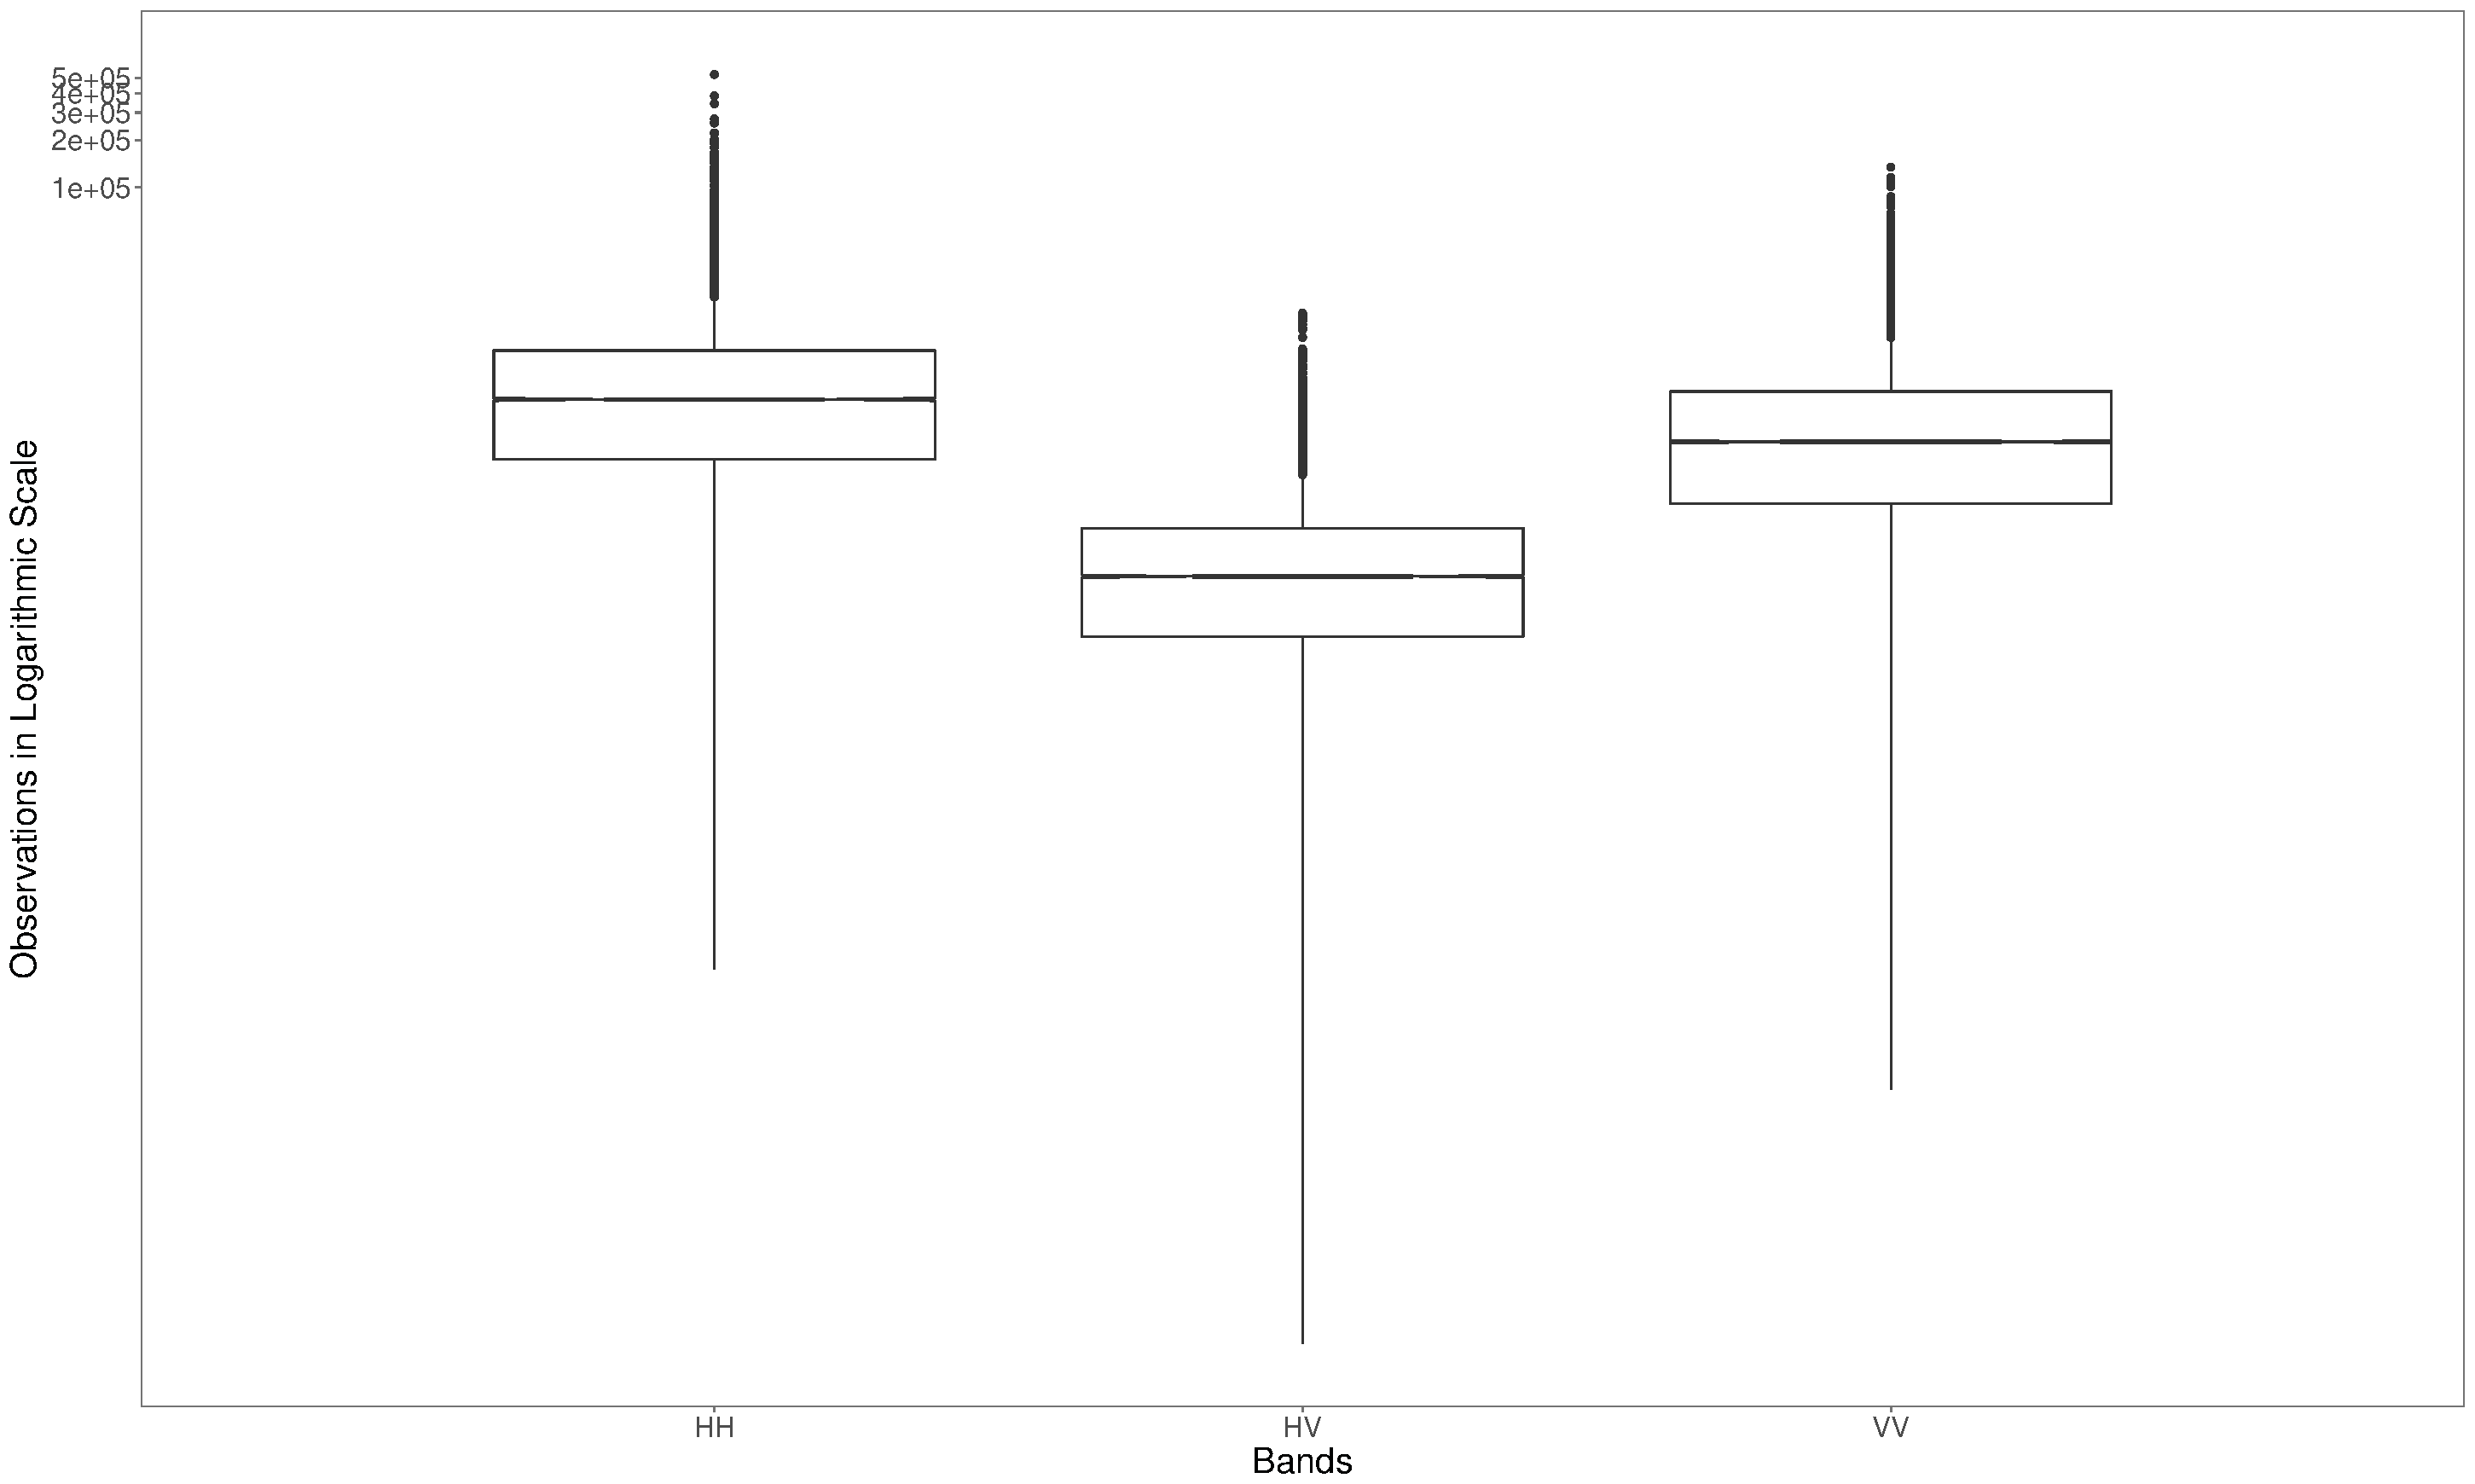
\includegraphics[width=\linewidth]{BoxPlotdark}
\caption{Boxplot of the three bands from the \texttt{dark} image}\label{Fig:BoxplotDark}
\end{figure}

Fig.~\ref{Fig:BoxplotDark} depicts what the \texttt{summary} command had revealed already, but it also provides strong evidence in favor of highly skewed data.
We were aware of this from Fig.~\ref{Fig:FittedDarkRegion}.

\section{Visualization}

Image visualization is the operation that maps values into pixels\cite{IPVG:2008}.
This mapping may be to a screen or to a file.

SAR images often have a huge dynamic range.